\todo[inline]{For each thing you explain also say why you explain it, what role will it play later in this thesis}

\section{Clients and their needs}

\subsection{UCL}
As said before, market gardening is getting more and more interest from searchers these last years. The UCL is thus currently leading researches in this field. The university has recently bought an ancient farm and plan to do some research in market gardening on the fields around.\footnote{\url{http://fermedelauzelle.be}} The point of these researches is to gather data about the viability, efficiency and profitability of different gardening principles. There are many theories about gardening on small surfaces, but not that much researches on this topics and the efficiency of most of them have not been proven.
Hence, UCL would like a web application that would help them gather data from this forthcoming gardening project but also from gardens around the country.
From our meetings with UCL's searchers we have defined some requirements:
\begin{itemize}
\item The application should have a searcher backend to allow easy access to gardens' data
\item Users should be able to choose which pieces of informations they agree to share with the university
\item Every task should have a \emph{note} field so growers can give more details to everything they do.
\item Every task should have a \emph{duration} field in order to collect data on the time needed for each cropping.
\end{itemize}
\subsection{Market gardeners}
Before starting the project, we met several vegetable grower in order to have their opinion on the application and their advice. As the application is intended to help them, it was essential to meet them. From these meetings, we defined what were their requirements:
\begin{itemize}
\item The application should help them in their planning
\item In order to help their planning, the application should remind them about cultural operations
\item The application should give them information about the previous years and their previous harvests
\item The application should have an economical side: one should be able to see which cropping is the most profitable.
\end{itemize} 
%\paragraph{Meetings}

\section{Vocabulary in software engineering}
In this section, we define some concepts specific to software engineering. These concepts will be used in the following sections. This section can be skipped by experts of the subject.
\paragraph{Agile Methodology}\label{par:agilemethodology}
The Agile methodology is a set of techniques and principles for conducting a development project. The main principle is to iterate over short periods (called sprints) divided in subphases in order to build the final product in an incremental way.
A sprint lasts between one and two weeks and is divided as follows: 
\begin{itemize}
    \item At the start of each iteration, we plan with the client what we are going to do this iteration.
    \item Next step is to think about how to build a good design to achieve the objective
    \item Then, we develop the features
    \item After, we test these features. If we switch these last two steps, we apply what is called Test-Driven Development. With this methodology, a team write tests before developing the corresponding features, ensuring that the tests will cover all the cases
    \item At the end of each sprint, we meet the client again to validate the changes and new features, collect his feedback about the project's progress and to define together the future work.
\end{itemize}
A visual representation of this iterative approach is shown on figure \ref{fig:agile-methodology}


\begin{figure}
    \centering
    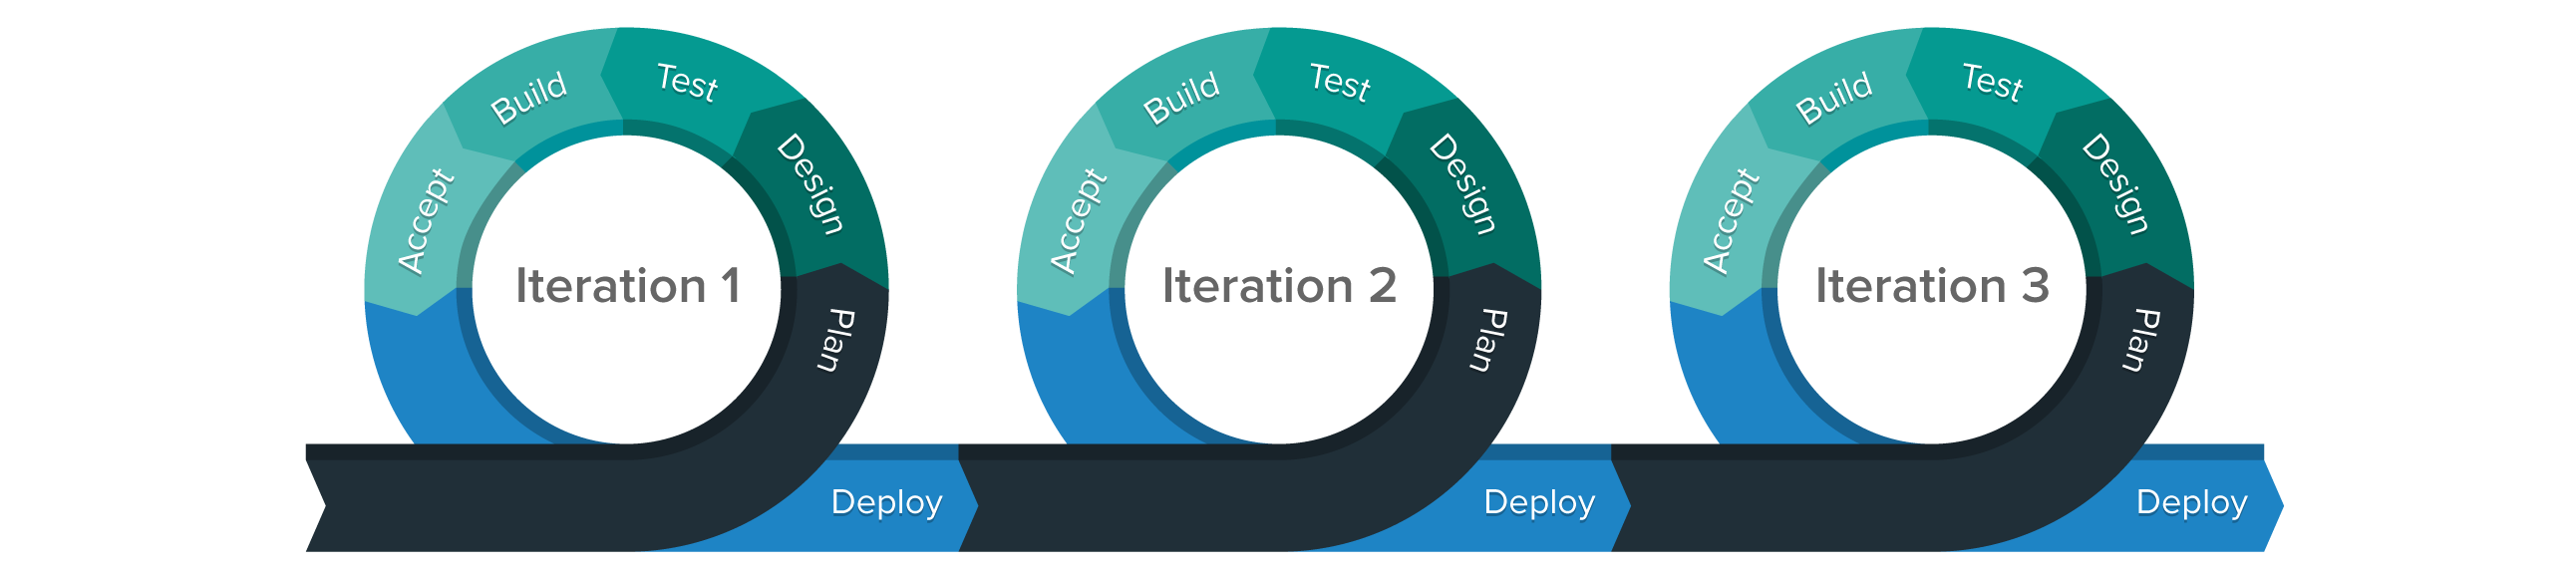
\includegraphics[width=\textwidth]{images/agile-methodolody.png}
    \caption{Iterations using Agile methodology}
    \label{fig:agile-methodology}
\end{figure}

A good summary of the Agile methodology is the agile manifesto\cite{agilemanifesto}, that states the main principles of this methodology.

\begin{bclogo}[logo=\bctrombone]{Agile Manifesto \cite{agilemanifesto}}
\emph{Individuals and interactions} over processes and tools.\\
\emph{Working software} over comprehensive documentation.\\
\emph{Customer collaboration} over contract negotiation.\\
\emph{Responding to change} over following a plan. \\
That is, while there is value in the items on
the right, we value the items on the left more.
\end{bclogo}

The main advantages of this methodology are to have flexibility and regular feedback on the product delivered.

\paragraph{Software framework}

%A framework is a set of tools that provides features that can be reused in multiple applications. 
\todo[inline]{Give clear definition of a framework}
A framework is different from a library in the sense that when using a library, we call the methods of the library while when using a framework, our code is called by the framework. The difference is shown on figure \ref{fig:framework-vs-library}. Frameworks help to build reusable and maintainable applications 
\todo[inline]{give some examples of frameworks + why you talk about it, integrate Django with it?}

\begin{figure}
    \centering
    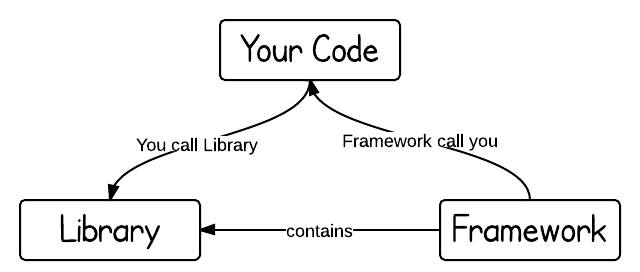
\includegraphics[width=0.5\textwidth]{images/framework-vs-library.png}
    \caption{Framework versus library}
    \label{fig:framework-vs-library}
\end{figure}


\paragraph{Object Relational Mapping}
\todo{here}

\paragraph{Continuous Integration}
Continuous integration (often referred as CI) is a software engineering practice to help development teams working on a set repository. 
When using CI, we automate a set of checks at each push request on a repository and developers should merge to this repository regularly. With continuous integration, we will detect bugs faster and more easily. We can also add tests to our continuous integration tool, these tests will then be run at each push request and we will receive a notification if they fail. Thanks to that, we can see exactly which commit implied a failure in the tests. If we do small regular commits, it will be really easy to find where the failure comes from.



\section{Which platform?}
First question to ask is which platform are we going to choose. We have two main clients; searchers at the UCL and gardeners. While searchers work mostly on their computer, gardeners spend most of their time on the ground and don't always have regular access to a computer. 
We could have think about a mobile application, but then we have to deal with different operating systems (Android and IOS mainly). For these reasons, we have opted for a web application. A web application is available on every device having access to internet, whatever the operating system is. With this solution we assure satisfaction of both clients.

%\section{Which licence}
%open source car par une volonté de rentabiliser le logiciel. L'interet étant d'avoir le plus de maraichers possibles pour récolter le plus de données possible du coté des chercheurs.

\section{Which methodology}
When this project began, we had no clear specifications about the final result to produce. The requirements have evolve during over weeks. Because of this incremental definition of requirements and specification, it was natural to follow and Agile methodology (see \ref{par:agilemethodology}).
As we were only one developer working on the project, we did not apply all principles of this methodology. We kept the iterative approach by doing regular meetings with the clients. We had meetings with the UCL client once a week and with a gardener once a month.
For each meeting, new features were presented to the client in order to have his approval (or not). These meetings were also the good moment to define priority for the coming weeks.


\section{Which languages?}
In this section we will analyse the different choices we had concerning all type languages. 
\subsection{Programming language}
To guide our selection of the perfect programming language we had several guidelines:
\begin{itemize}
\item As we want the application to be reusable and maintainable by future students or searchers from the UCL, we had to choose a language easy to learn and to understand, with a fast learning curve. From next year, first year student at the EPL faculty will be taught Python as first programming language. In the agronomy faculty, it is common that searchers use Python 
\item As we are targeting a web application, we needed a language with web frameworks available.
\item Because of the nature of our application and the requirements defined at the beginning of the project, we also wanted an object oriented language.
\end{itemize}

From these guidelines it was natural to choose \emph{Python} as programming language.
\paragraph{Python}
Python is a programming language used in many fields. Its main advantage is great readability. Its first release was in 1991 and its creator is Guido van Rossum. Python is an interpreted language which means there is no compilation stage before running the program. The interpreted executes it directly. This feature makes it fast and easy to use even for very small projects, but for bigger projects Python is known as being slow because there is no compilation optimisation possible.\cite{python-slow}
However, Python has a big active community and thus great support and documentation which makes it a reliable language. Python is currently at the fourth place of the TIOBE index \footnote{The TIOBE index measure the popularity of programming languages: \url{ https://www.tiobe.com/tiobe-index/}} which suggests that Python is a good choice of programming language. 

\subsection{Web framework}
From the previous choice, we already narrowed the range of available web framework.
Besides Python as requirement, the principal guidelines for the choice of a web framework were the following:
\begin{itemize}
\item It should be easy to use and understand as we have chosen Python partly for its readability
\item It should be stable and reliable, so with a good documentation and a community behind reporting bugs and keeping the framework up to date.
\item It should have basic web features such as authentication, we do not want to reinvent the wheel and reimplement existing modules. 
\end{itemize}
From these guidelines, we spotted 4 popular Python web frameworks (figure \ref{fig:webframeworks}) Pyramid\footnote{\url{https://trypyramid.com/}}, Bottle\footnote{\url{http://bottlepy.org/docs/dev/}}, Django\footnote{\url{https://www.djangoproject.com/}} and Flask\footnote{\url{http://flask.pocoo.org/}}.

\begin{figure}
\centering
\begin{subfigure}{.24\textwidth}
  \centering
  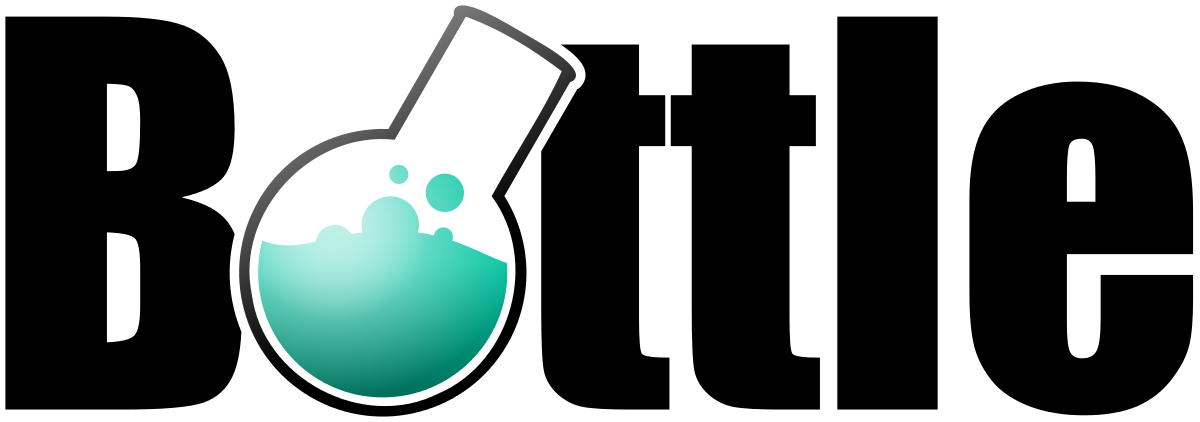
\includegraphics[width=0.8\linewidth]{images/bottle.png}
\end{subfigure}%
\begin{subfigure}{.24\textwidth}
  \centering
  
\includegraphics[width=0.8\linewidth]{images/pyramid.png}
\end{subfigure}
\begin{subfigure}{.24\textwidth}
  \centering
  
\includegraphics[width=0.8\linewidth]{images/flask.png}
\end{subfigure}
\begin{subfigure}{.24\textwidth}
  \centering
  
\includegraphics[width=0.8\linewidth]{images/django.png}
\end{subfigure}
\caption{Four popular Python Web Framework}
\label{fig:webframeworks}
\end{figure}


Bottle and Flask are more intended for small projects and do not offer lots of support for bigger applications with more needs. For example, they don't have a built-in authentication module. Their key advantages are their small size and their fast installation. We dropped those choices (and other similar lightweight web framework) early on.
Django and Pyramid are both designed to create web applications of medium to large size.  They are both open source and have a large community.
The main difference between Django and Pyramid is while the later is a lightweight framework, the former is a high-level web framework. This imply that Pyramid, compared to Django, is well-known as being a lot more flexible.
There is not a framework better than the other, they have different features and we have to choose which ones are the most important for us in our project.
We did not choose Pyramid because we did not need the flexibility it offers.

Finally, we opted for Django because of its maturity, its popularity and its wide range of built-in modules. We relied upon its ORM\footnote{Object Relational Mapping}, its authentication module, its administration interface, its MVT\footnote{Model View Template} design pattern and others features that will be discussed in the later chapters about implementation.


\subsection{Query language}
Once again, the choice of Django reduces the choices we have concerning the database we are going to use. First of all, Django does not officially support NoSQL databases.
Official documentation is only given for PostgreSQL, MySQL, SQLite and Oracle databases.
Our choice was made between PostgreSQL and MySQL because SQLite is intended for small databases and Oracle is not a free alternative.
Once again, PostgreSQL and MySQL have both their own advantages. We've choose PostgreSQL because it is the most popular relational database management system (RDMS) with Django.

\subsection{Written language}
Code (including tests) has been written in English for a better readability. But all textual information on the website are in French. This has been decided because our two clients speak French.

\section{Maintenance}



\todo[inline]{Why you explain this, what CI you use, what CI features and tools you use; why you use these}